%%%%%%%%%%%%%%%%%%%% author.tex %%%%%%%%%%%%%%%%%%%%%%%%%%%%%%%%%%%
%
%%%%%%%%%%%%%%%% Springer %%%%%%%%%%%%%%%%%%%%%%%%%%%%%%%%%%

\title*{Using Graph Databases to Explore the Dynamics of Genetic Programming Runs}
% Use \titlerunning{Short Title} for an abbreviated version of
% your contribution title if the original one is too long
\author{Nicholas Freitag McPhee, David Donatucci, and Thomas Helmuth}
% Use \authorrunning{Short Title} for an abbreviated version of
% your contribution title if the original one is too long
\institute{Nicholas Freitag McPhee \at Division of Science and Mathematics, University of Minnesota, Morris, MN USA
\and David Donatucci \at Division of Science and Mathematics, University of Minnesota, Morris, MN USA
\and Thomas Helmuth \at Computer Science, University of Massachusetts, Amherst, MA USA}

\maketitle

\abstract{
	For both practical reasons and those of habit, most evolutionary computation research is presented in highly summary
	form. These summaries, however, often obscure or completely mask the profusion of specific events such as selections, crossovers, and mutations
	that are ultimately responsible for the aggregate behaviors that we're interested in. In this chapter we take an almost
	opposite approach and use the Neo4j graph database system to record and analyze the entire genealogical history of 
	a set of genetic programming runs. We then explore a few of these runs in some detail, discovering some important
	properties of lexicase selection that may help us better understand the dynamics of lexicase selection and the considerable
	ways in which it differs from tournament selection. More broadly, we illustrate the value of recording and analyzing this
	level of detail, both as a means of understanding the dynamics of particular runs, and as a way of generating questions
	and ideas for subsequent, broader study.}

\begin{keywords}
keywords to your chapter, these words should also be indexed
\end{keywords}
\index{keywords to your chapter}
\index{these words should also be indexed}
\\

\section{Introduction}
\label{sec:introduction}

It is common practice in empirical evolutionary computation (EC) 
research to perform a substantial number of runs, and then 
report a handful of aggregate statistics at the end that summarize and (hopefully) represent 
the complex interactions and dynamics of those many runs. Tables present values such 
as mean or median best fitnesses at the end of runs, collapsing the complexities of dozens or 
hundreds of runs into a single number, possibly with a standard deviation or (even better) a 
confidence interval to give a sense of the distribution. Plots can often be more informative, 
showing, for example, how these numbers change over time during the runs, possibly giving a sense of 
the system dynamics and the range of behaviors. These plots, however, are typically still aggregate representations that
that obscure or completely hide important moments that, if explored, might reveal valuable insight into the 
evolutionary dynamics being reported.

An alternative would be to collect, store, and analyze at least some of the rich panoply of 
evolutionary and genealogical events that make up the vital low-details details of these runs. 
Databases provide a natural tool for 
storing and accessing the data, but traditional relational
databases are poorly suited for a variety of queries that are important for the genealogical analysis
we need for exploring the evolutionary dynamics of our EC runs.
In this chapter, we illustrate the use of graph databases as an alternative storage and analysis tool for
evolutionary computation runs. We have previously demonstrated that graph databases
can be an effective tool for analyzing complex genetic programming (GP) dynamics \citep{donatuccianalysis}, which led directly
to a proposed change to standard sub-tree crossover in tree-based GP, \citep{mcphee:GECCO15}.
Here we will use the open source Neo4J graph database tool\footnote{\url{http://neo4j.com/}} 
to explore data from a
collection of PushGP runs \citep{Helmuth:2015:GPTP} on several problems drawn from a benchmark collection of introductory 
programming problems \citep{Helmuth:2015:GECCO}.

Note that this is \emph{not} going to be a presentation of ``traditional hypothesis-driven 
research''. It will be based on an \emph{assumption}, namely that something interesting happens in
these runs, and that we can learn useful things by exploring them in more detail, but the presentation
will be fairly discursive, reflecting our back-and-forth experience of wrestling with the data. Our
initial queries start from fairly obvious questions (e.g., ``Why did we succeed here?''), but from
there we engage in a dialog with data, letting the answers to early questions shape and guide our 
subsequent exploration. We are not presenting a tidy, sterile summary of our adventures, but
the messier (but we think more informative in this context) journal of what Pickering might call
our ``mangle of practice'' \citep{smith2008mangle, pickering:AJS:1993}.

Here we explore the impact of lexicase \citep{Helmuth:2015:ieeeTEC} and tournament selection 
on a dynamics of runs whose aim is to solve a basic software synthesis problem. 
In the process of this ``mangle'' we are able to discover surprising and likely important properties of
lexicase that suggest areas of additional, broader (more ``statistical'') exploration and indicate reasons
for the substantially better performance seen when using lexicase on a variety of software synthesis 
problems \citep{Helmuth:2015:GECCO}.

Because we're going to focus on the use of a graph database to explore this data, there will
on occasion be avenues of exploration that we won't pursue here because they would properly involve
different tools. This exploration raises obvious and important questions about the relationships between,
for example, parent and child genomes. These would be best addressed using things like 
difference-merge tools from software engineering, or sequence alignment tools from genomics.
Entire papers could be written on the use of those tools in this context, but we'll consider that
beyond the scope of this chapter. Our queries in the graph database will, however, help us identify key moments
and individuals in the course of a run, pointing out particular places where we should focus those tools. There are thousands
of potential genome comparisons to make in a single run, for example, but our graph databases analysis helps identify
some of the critical individuals, crossovers, and mutations in the run, allowing us to concentrate on the
steps that are likely to have mattered most in the success of a evolutionary run.

We'll provide expanded motivation for this work in Section~\ref{sec:motivation}, and background on relevant tools
and concepts in Section~\ref{sec:background}. In Section~\ref{sec:lexicaseRun} we explore in some detail a successful
lexicase selection run, identifying several interesting properties of lexicase selection that strongly distinguish it from
other, more traditional selection methods, and in Section~\ref{sec:tournamentRun} we compare those to results of 
an exploration a successful tournament selection run. After these detailed explorations of individual runs, in
Section~\ref{sec:cumulativeResults} we step back a little and look at the results of expanding some of our queries
across hundreds of runs, and then wrap up with some conclusions in Section~\ref{sec:whatDidWeLearn}.

\section{Motivation}
\label{sec:motivation}

Consider the job of a paleontologist, who regularly reconstructs not just individuals but also
species and entire phylogenetic trees on the basis of handful of teeth and bones, or even just
impressions left in prehistoric mud. They rarely have DNA, so any evolutionary relationship is
inherently speculative, subject to constant debate and revision. Even with detailed DNA sequences,
the construction of phylogenetic trees for existing species is a challenge.

%\marginpar{A reference
%	for all of this phylogenetic reconstruction stuff would be useful.}

In evolutionary computation, however, we have access to \emph{everything}, at least in principle. Every
selection, every mating, every mutation, and every crossover happens in our code and on our watch.
Yet we typically throw almost all that data away, reporting just aggregate statistics and summary
plots, completely failing to take advantage of our privileged position, a position most 
paleontologists would presumably eye with considerable envy. Not only does this seem an inherent
waste, these aggregations typically obscure critical moments in the dynamics of runs which might
speak volumes if explored.

%\marginpar{Perhaps include a sample plot and show how it hides things? One of Tom's 
%	diversity or cluster plots? A synthetic plot? Maybe that's just not necessary?}

While this sort of aggregate reporting is often valuable, allowing for important comparative
analysis of, for example, the impact of different genetic operators, it typically fails to provide
any sense of the \emph{why}. Yes, Treatment A led to better aggregate performance than 
Treatment B -- but what happened in the runs that led to that result? Any success at the end of a
run is ultimately the intricate combination of hundreds or thousands of selections, recombinations
and mutations, and if Treatment A is in some sense ``better'' than Treatment B, it must ultimately
be because it affected all those genealogical and genetic events in some significant way, biasing them
towards events that made success more likely.

Unfortunately, published research very rarely includes information that might shed light on 
these \emph{why} events. We rarely see evolved programs, for example, or any kind of post-run analysis
of those programs, and there is almost never any data or discussion of the genealogical history that
might help us understand how a successful program actually came to be. 
Sometimes these events and details aren't included
for reasons of space and time; evolved programs, for example, are often extremely large and complex,
and a meaningful presentation and discussion of such a program could easily take up more space than
authors have available given the typical space limitations in published work.
Our suspicion, however, is that another reason this sort of \emph{why} analysis often isn't 
reported is because it isn't done, in no small part because it's hard. As EC researchers we're in the
``privileged'' position of being able to collect anything and everything that happens in a run, 
but that's a potentially huge amount of data, and leaves us with two substantial problems: 
How to \emph{store} the data, and how to \emph{analyze} the data
after it's stored. 
Decreasing data storage costs have done much to mitigate the first problem.
If, however, one collects a very rich data set it's still easy to quickly generate terabytes of data,
and even if one has a place to put the data, one still needs reasonable tools to analyze the data.

Assuming one has access to the necessary gigabytes or terabytes of storage, 
databases are the obvious tool for the collection of the data. Most common database structures and tools,
however,
don't lend themselves to the kinds of analysis that we want and need in evolutionary computation work. 
Most relational and document-based databases, for example, require complex and expensive 
recursive joins to trace significant hereditary lines, making this approach increasingly unfeasible.
In exploring the dynamics of an EC run, it is necessary to
make connections across dozens or even hundreds of generations, which simply isn't plausible with a
relational database \citep{Robinson:GraphDB:Book}. 
While we use Neo4j as our graph database in this work, there are 
numerous other 
graph databases that could potentially be effective tools \citep{wiki:GraphDB}. We make no claims
to have exhaustively explored the range of possible database tools for this sort of work.

\section{A little background on tools and problems}
\label{sec:background}

This section provides some background on some of the key subjects of this work:
\begin{itemize}
	\item The Neo4J graph database and its query language Cypher
	\item The PushGP system
	\item Lexicase selection
	\item The replace-space-with-newline test problem
\end{itemize} 

\subsection{Neo4J and Cypher}
\label{subsec:Neo4j}

Graph databases \citep{Robinson:GraphDB:Book} are a relatively new database tool, where data is stored 
as a collection of nodes and relationships in a graph, with a specialized query language that makes 
it easy to ask questions about complex relationships. In Neo4j, information is stored using
vertices and edges, commonly referred to as nodes and relationships, 
respectively. Neo4j also allows properties to be stored in both nodes and edges.
In our work, nodes typically represent individuals, and \texttt{:PARENT\_OF} relationships 
capture the central genealogical connections. We store important data such as the total error as
properties of individual nodes, and genetic operators as properties on 
\texttt{:PARENT\_OF} edges.\footnote{In practice we also include nodes to represent things
	such as runs and generations, using these to store relevant cumulative information.}

The Neo4j query language, Cypher, allows this data to be readily extracted from the Neo4j database.
A detailed description of Cypher is beyond the scope of this chapter, but Cypher's central feature is
the ability to describe patterns using ``ASCII art''. The Neo4j engine can then search
the graph for subgraphs matching these patterns. Cypher also provides the ability to 
filter results based on properties in a manner quite similar to more traditional SQL queries.

\subsection{PushGP}

PushGP \citep{spector:2002:GPEM, 1068292} is a stack-based genetic programming system. The details
of PushGP aren't crucial for this analysis as we're going to focus on the behavioral properties of
individuals in this work, but it useful to know a few things:
\begin{itemize}
	\item PushGP uses a linear genome, which is then converted into a program as described below.
	\item PushGP supports a variety of \emph{typed} stacks, with corresponding typed instructions.
	The \texttt{string-pop} instruction, for example, pops the top of the \texttt{string} stack,
	and the \texttt{integer-add} instruction takes the top two items from the \texttt{integer}
	stack, adds them, and pushes the result back onto the \texttt{integer} stack.
	\item There is a \texttt{exec} stack which can hold blocks of instructions. This is what allows
	PushGP programs to loop or recurse, as pushing a block of instructions onto the \texttt{exec}
	causes those instructions to be executed next.
\end{itemize}

The PushGP system used here uses \emph{Plush genomes}, which are linear genomes consisting of 
instructions paired with \emph{closed counts}. The close counts are natural numbers 
indicating how many open code blocks should be closed after this instruction. Several instructions
that are typically used with blocks of code in human programming, such as conditionals and loops,
have an implicit ``open block'' that is translated into an explicit ``open block'' when the genome
is converted to a Push program. The close counts, then, are necessary to allow the PushGP
system to evolve the desired ``end block''s.

In the runs explored here, there are three genetic operations:
\begin{itemize}
	\item alternation
	\item uniform-mutation
	\item uniform-close-mutation
\end{itemize}
Alternation is similar to an N-point crossover in genetic algorithms. The two parent genomes
are traversed from left to right taking instructions from one or the other for the child, with
a small probability at each instruction of switching which parent is being used as the instruction
source. When an alternation event happens, there's a small amount of gaussian noise added to the
instruction location; how much deviation is possible is controlled by an \emph{alignment deviation} 
parameter.

Uniform-mutation simply replaces each instruction with a randomly chosen instruction with some
small probability. Uniform-close-mutation modifies each close count value with some small probability.
The runs discussed here allowed for \emph{pipelining} of genetic operators, so we might have
combinations like alternation followed by uniform-mutation.

For additional details and the particular parameters used in these runs see \citep{Helmuth:2015:GECCO}.

\subsection{Lexicase selection}

Pseudocode for the lexicase selection algorithm is outlined in 
Algorithm~\ref{alg:lexicase}. In each parent selection event, the lexicase selection algorithm 
first randomly orders the test cases. It then eliminates any individuals in the population 
that do not have the best performance on the first test case. 
Assuming that more than one individual remains, it then loops, eliminating any individuals from 
the remaining candidates that do not have the best performance on the second test case. This 
process continues until only one individual remains and is selected, or until all test cases 
have been used, in which case it randomly selects one of the remaining individuals.

\begin{algorithm}[tb]
	\begin{algorithmic}
		\STATE \texttt{candidates} $:=$ the entire population
		\STATE \texttt{cases} $:=$ list of all the test cases in a random order
		\WHILE{$|\texttt{candidates}|>1$ \AND $|\texttt{cases}|>0$}
		\STATE \texttt{current}, \texttt{cases} := $\textrm{first}(\texttt{cases})$, $\textrm{rest}(\texttt{cases})$
		\STATE \texttt{best\_performance} $:= \min \{ \textrm{perf}(i, \texttt{current}) \;|\; i \in \texttt{candidates} \}$
		\STATE \texttt{candidates} := $\{ i \;|\; i \in \texttt{candidates} \;\land\; \textrm{perf}(i, \texttt{current}) = \texttt{best\_performance}\}$
		\ENDWHILE
		\RETURN random individual from \texttt{candidates}
	\end{algorithmic}
	\caption{Psuedocode for the lexicase selection algorithm. The use of $\min$ when computing 
		\texttt{best\_performance} assumes that the goal is to minimize on each test case, which
		is true in the work presented here, where the goal for all test cases is to minimize error.
		This can be easily generalized to other settings.}
	\label{alg:lexicase}
\end{algorithm}

The central properties of lexicase selection are that (a) it doesn't combine all the errors into a single
fitness value and (b) because of the random ordering of test cases, every test case is likely to be
most important (first to be considered) at least occasionally. With a population of 1,000 individuals
and a problem with 200 test cases, for example, we would expect each test case to be first several
times in each generation. The hope, then, is that this ensures some diversity in the population, with
different (groups of) individuals being rewarded for their ability to perform well on different test
cases.

\subsection{Replace-space-with-newline}

The replace-space-with-newline problem is an introductory programming benchmark problem taken
from~\citep{Helmuth:2015:GECCO}. In this problem the program is given an input string and required to
both (a) print the string with all the spaces replaced by newlines and (b) return an integer that
is the number of non-space characters in the input string. There are 100 different training instances 
for this problem, each of which generates two error values: One is the Levenshtein distance between
the printed output and the target print string, and the other is the absolute difference between
whatever value is on the top of the \texttt{integer} stack and the expected return value. A penalty
value of 1,000 is assigned for test cases that were expecting a return value but found the
\texttt{integer} stack empty.

For tournament selection runs, all 200 of these error values were added together to form the
total error, which was used as the fitness for the individuals. For lexicase selection the errors
were kept separate in an error vector of 200 values; this, as we shall see, frequently allowed individuals to be selected who did 
well on some test cases, but very poorly on others.

\subsection{Our data}
\label{sec:ourData}

The data we explored in this paper is a subset of the data collected for \citep{Helmuth:2015:GPTP}. In particular
we have the full genealogical records for one hundred runs of the replace-space-with-newline problem using each 
of lexicase selection and tournament
selection with tournament size 7. In those
runs, 57 of the 100 lexicase runs succeeded in the sense that an individual was discovered that had zero
error on all 200 of the training cases. Tournament selection with tournament size 7 only
had 13 successes out of 100 runs, so it seems that
lexicase selection provides a significant advantage on this problem. Similar results in \citep{Helmuth:2015:GECCO}
indicate that lexicase is in fact generally much more successful across a broad range of
software synthesis problems than either tournament selection and implicit fitness
sharing and tournaments.

\section{Lexicase, meet Replace-space-with-newline}
\label{sec:lexicaseRun}

% This is run 6, lexicase, replace-space-with-newline.

It's one thing to know that lexicase succeeds 57 out of 100 times on the replace-space-with-newline problem, but that
leaves us with the crucial question of \emph{why}? In order to answer this question, we chose one successful 
run to explore in more detail.
We're making no claims that this is a ``representative'' run (whatever that would even
mean); it's an \emph{interesting} run, though, and our hope is that by understanding its dynamics
better we can learn useful things about both the problem and the tools we're applying. Looking at this run in some
detail certainly unearthed several surprising results, and in Section~\ref{sec:cumulativeResults}
we'll expand our view by looking at some cumulative results across all hundred runs.

\subsection{Hey, we won! But how did we get there?}

\begin{figure}[tp]
	\begin{center}
	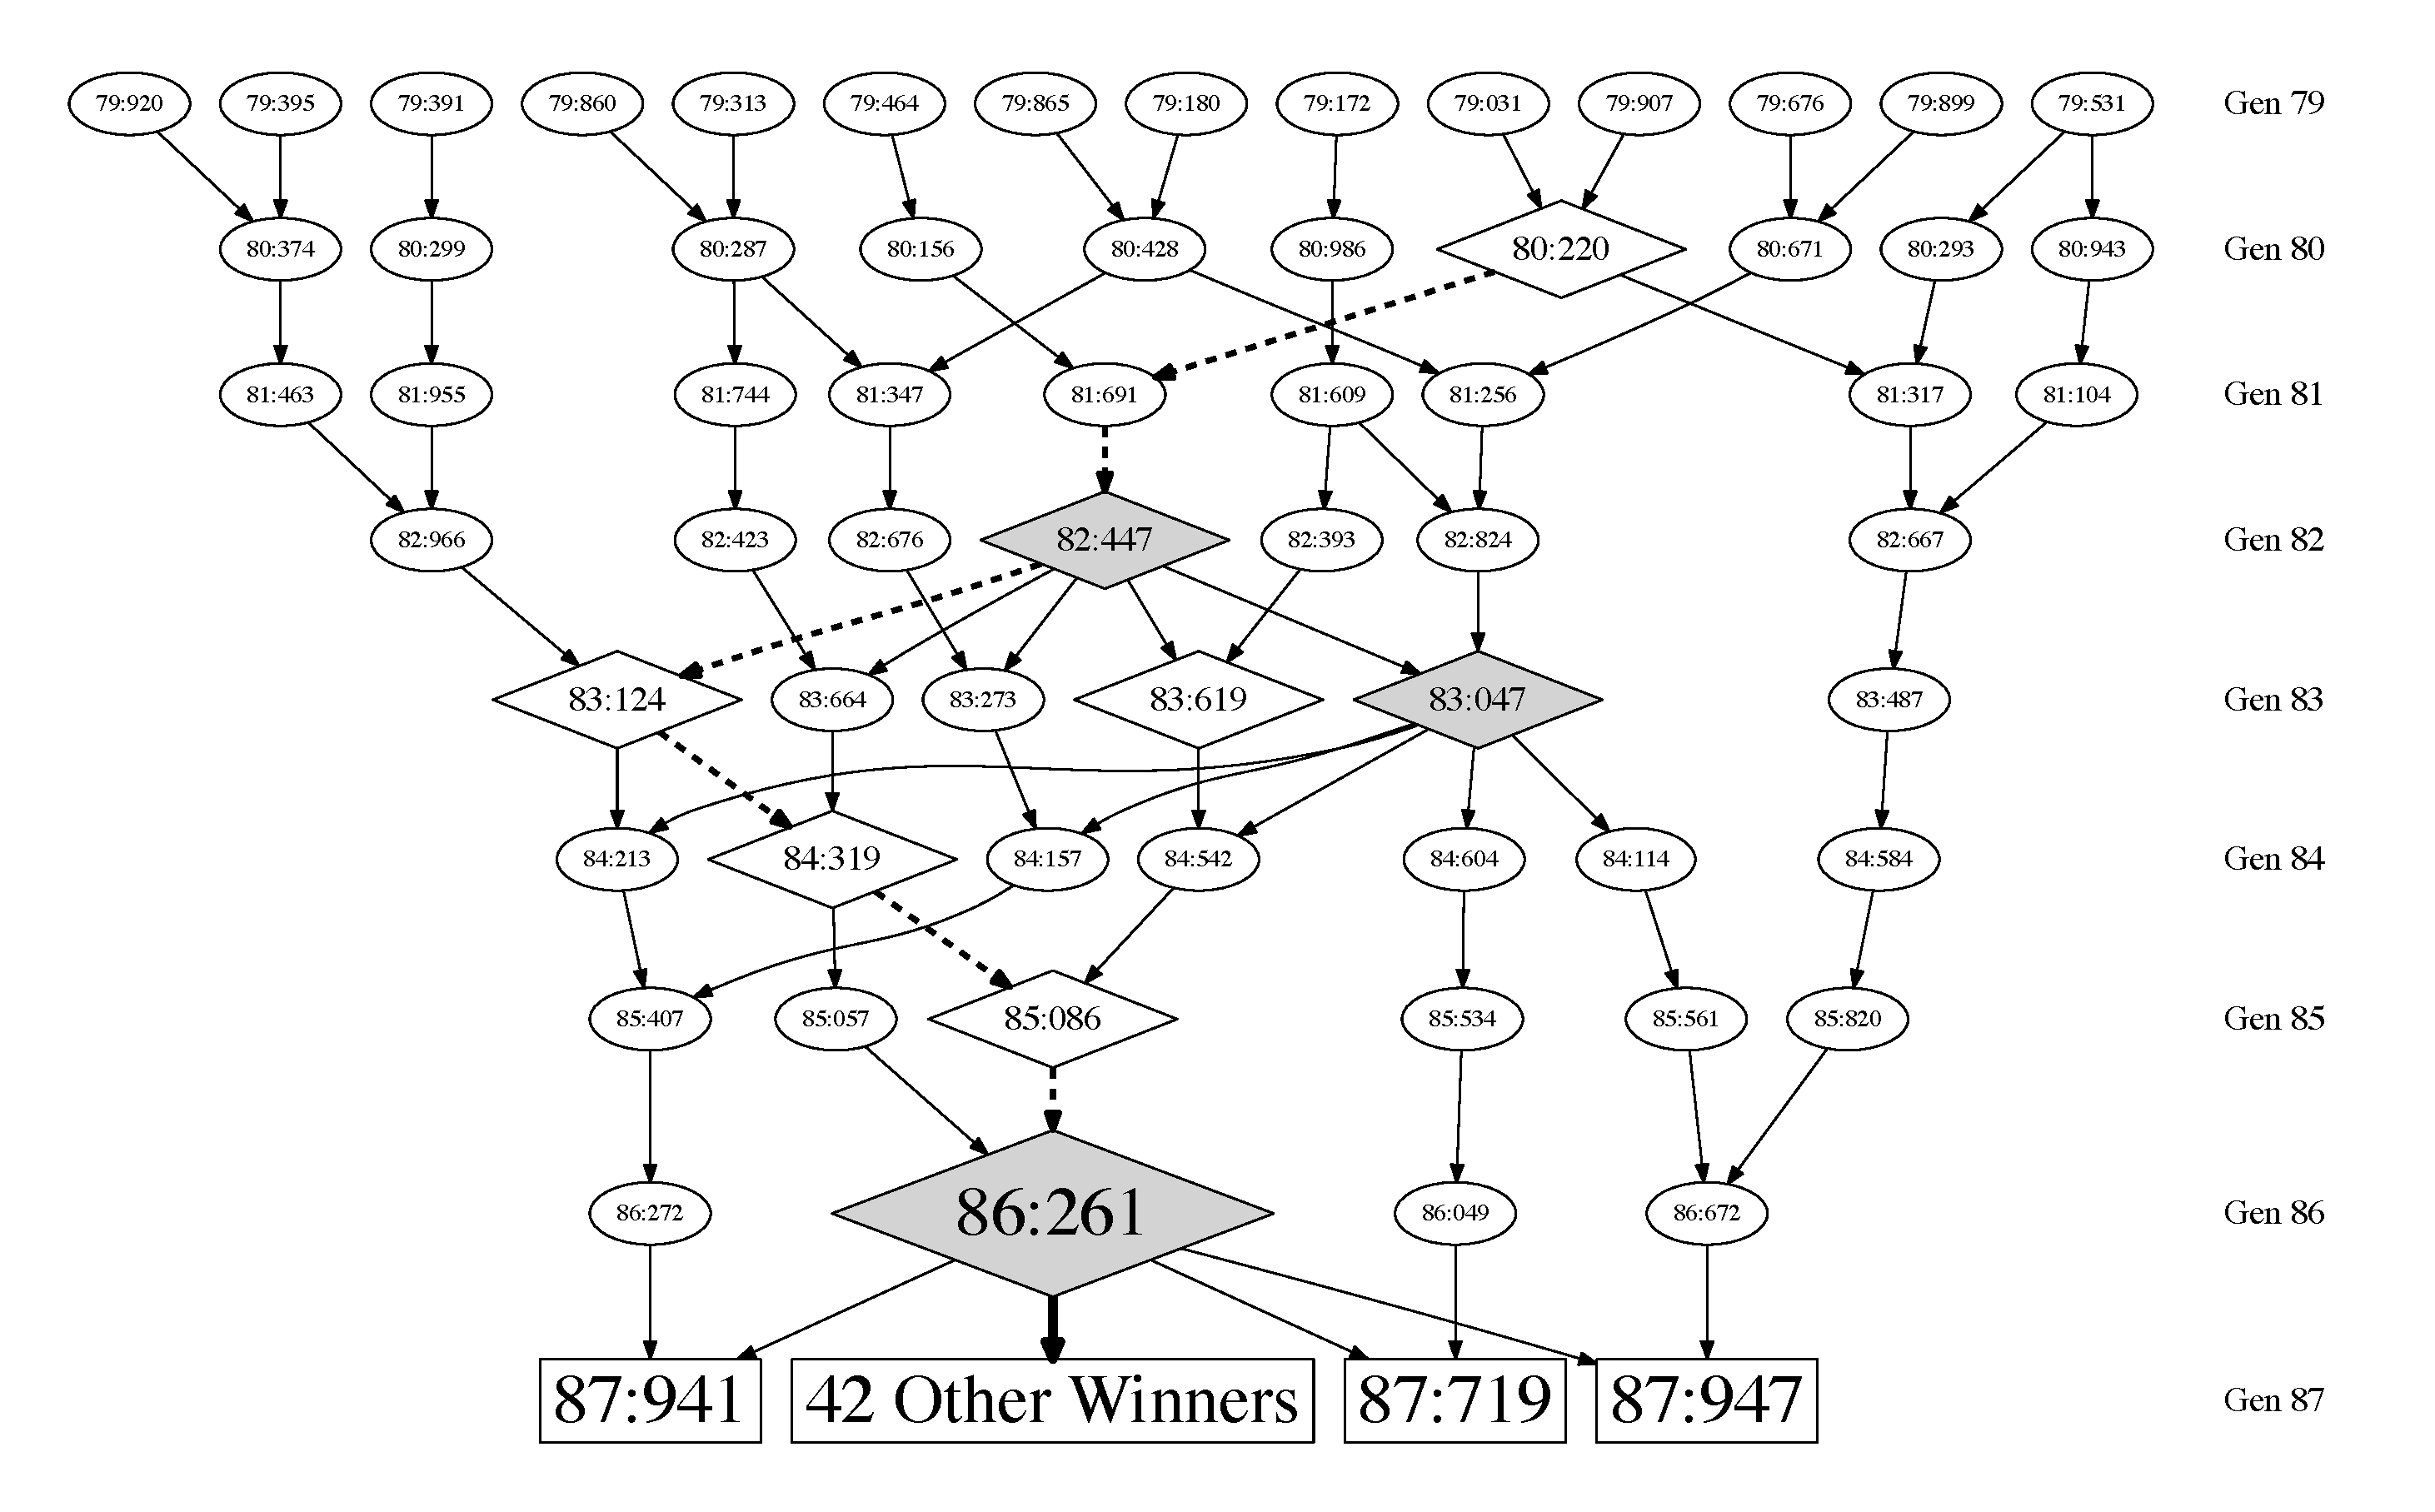
\includegraphics[width=0.9\textwidth]{figures/ancestors_of_winners_colons.pdf}
	\end{center}
	\caption{Ancestry of the 45 ``winners'' from run 6 of lexicase, replace-space-with-newline. Nodes
		with diamonds instead of ellipses had an unusually large number of offspring. Shaded nodes
		had an unusual number of offspring that were ancestors of winners. The dashed lines highlight
		individuals that had an unusually large number of distinct ancestry paths down to a winner.
		See the text for more details}
	\label{fig:winnerAncestors}
\end{figure}

A natural place to start our analysis of this run is at the end, when the GP system created one or more individuals that 
solved the problem. So we used Neo4J to find all the ancestors of any ``winning'' individual, i.e., an individual with a total error of 
on all 200 test cases. Using Cypher, we can easily ask for this subset
of the population going back to generation 79.\footnote{We could certainly 
	have gone back farther in time, but the graph would have become impossible to read as the
	number of nodes would have ballooned from a few dozen to hundreds or thousands. We went
	back to generation 79 because that was the most recent generation that had more than 10
	distinct ancestors of a winning individual.}

Figure~\ref{fig:winnerAncestors} shows the ancestry of all of the winners from generation 87 
(when we first found a winner in this run) back to generation 79.
Each node in the graph represents an individual, and each directed edge indicates a parent-child
relationship, with the edge going from the parent to the child. The numbers inside the nodes are
Neo4J internal IDs; we'll use these as ``names'' for the individuals as we tell the stories 
we uncover.\footnote{We actually assign each individual a UUID so we can combine multiple runs, but
	the Neo4J IDs are shorter and easier to use in our story telling.} Each ID has two parts:
the part before the colon is that individual's generation, and the part after is effectively
just a random three digit identifier.

Ignoring for the moment the adornments (shape, shading, etc.), there are several things that
we can observe right away:
\begin{itemize}
	\item There are 45 distinct winners in the final generation, or 4.5\% of the population of
	1,000 individual. This tells us that constructing a winner from the individuals in generation 86
	wasn't entirely trivial, but it also wasn't a huge challenge and happened multiple times.
	\item The 45 winners only had four distinct ancestors in the preceding generation.
	\item All 45 winners had a single individual (86:261, marked with a large shaded diamond near
	the center bottom) as at least one of their parents, and 42 of
	them had 86:261 as their \emph{only} parent, i.e., they were mutations of 86:261, or were the result
	of self-crosses of 86:261. To simplify the graph, we've combined those 42 individuals into a
	single node labeled ``42 Other Winners''.
	\item The number of ancestors of winners doesn't grow quickly as we move back in time. We have to
	go back to generation 80 to find 10 individuals (or 1\% of the population) that are ancestors of
	winners, and in generation 79 there are still only 14 ancestors of winners. In fact, we have to
	go trace the ancestry all the way to generation 63 to find a time where over 100 individuals (or over 10\% of 
	the population) were ancestors of a winning individual.
\end{itemize}

\subsection{Surprising fecundity (especially given that total error)}
\label{sec:surprisingFecundity}

Looking at Figure~\ref{fig:winnerAncestors} we can see that a few individuals have more offspring
represented than others. As we've already mentioned, individual 86:261 has 45 successful offspring,
and both individuals 82:447 and 83:047 have five offspring in the graph, i.e., five offspring that were
ancestors of a winning individual in generation 87. Each of these is marked in 
Figure~\ref{fig:winnerAncestors} with a shaded diamond.

Figure~\ref{fig:winnerAncestors},
however, only tells us how many offspring an individual had that were themselves either a winner
or an ancestor of a winner, as no other nodes are displayed. One
might, however, wonder how many total offspring an individual has
regardless of whether they were a winner or not. Using a Cypher query to identify the most
fecund ancestors of winners in these last nine generations, reveals several things that were
quite surprising (at least to some of the authors). The most remarkable of these was that individual 86:261 
was a parent of 934 of the 1,000 individuals in generation 87! Given that lexicase selection was
designed in significant part to spread selection events out across the population, this makes it
clear that there are times when lexicase does the opposite, and instead puts nearly all its eggs in
a single basket. This level of selection focus would simply be impossible using almost any other
common type of selection such as tournament selection; in most uses of tournament selection, 
for example, no individual can be in more than a relative handful of tournaments, and thus can't be
a parent terribly often no matter how fit they are.

While no other node in Figure~\ref{fig:winnerAncestors} has nearly as many children as 86:261 did,
there are several that also had very high reproduction rates, putting them well above what would be 
possible with something like tournament selection. Individual 82:447, for example, had
443 offspring, including the 5 illustrated in Figure~\ref{fig:winnerAncestors}. In fact there were
eight individuals in Figure~\ref{fig:winnerAncestors} that have more than 100 offspring; each of
these is indicated with a diamond shape. This highlights a particularly
interesting ancestry chain from 80:220 through 81:691, 82:447, 83:124, 84:319, 85:086 to 86:261, marked with
dashed edges in Figure~\ref{fig:winnerAncestors}. With the exception of 81:691, which ``only'' had 17
offspring, each of these seven individuals had more
than 100 offspring, and thus had a fairly dominate role in shaping the generation that followed them. 

If we look at the total error in of the individuals in Figure~\ref{fig:winnerAncestors}, we again
find some significant surprises that tell us quite a lot about lexicase selection. In particular, if
we look at the total error for each individual along the dashed path from 80:220 through
82:447 to 86:261, the total errors of the first five
individuals in the chain are reasonably low. One (individual 82:447) has the best total error in
that generation and all but 81:691 (the individual with only 17 offspring) are in the top fifth of the 
population when ranked by total fitness. The fitnesses 
of the last two (the grandparent and parent of \emph{every} one of the 45 solutions), however, 
came as quite a shock. In particular, individual 85:086 has a total error of 100,000, placing it
\emph{very near the bottom of the population by total error} (rank 971). Individual 86:261, which was
the parent of 924 of the 1,000 individuals in the next generation, has a total error of 4,034, placing
it below $3/4$ of the population in its generation by that aggregate measure.

\begin{table}[t]
	%\sidecaption[t]
	\caption{The total error and rank (by total error) in the population in that individual's generation
		for the sequence of ``diamond'' individuals from in Figure~\ref{fig:winnerAncestors}.}
	\label{table:winnerFitnesses}
	\begin{center}
	\begin{tabular}{rrr}
		Individual & $\quad$ Total error & $\quad$ Rank in population \\
		\hline\noalign{\smallskip}
		80:220 & 321 & 147 \\
		81:691 & 441 & 268 \\
		82:447 & 107 & 1 \\
		83:124 & 157 & 85 \\
		84:319 & 240 & 188 \\
		85:086 & 100,000 & 971 \\
		86:261 & 4,034 & 765
	\end{tabular}
	\end{center}
\end{table}

So how could individuals with such terrible total fitness end up being selected so often as parents?
Exploring the specific test case errors reveals that individual 85:086 is perfect on half of the test
cases (all those that involve printing), but gets a penalty error of 1,000 on the other half, presumably
because it never actually returns a value. Every one of its ancestors in 
Table~\ref{table:winnerFitnesses}, however, has at least a few non-zero errors on the printing
test cases, meaning that any lexicase ordering that places a few key printing test cases before
any of the ``return'' test cases would likely select individual 85:086.

What about individual 86:261, with it's 934 offspring? It is perfect (has error zero) on 194 of the 200
test cases, with it's total error of 4,034 coming from the remaining 6 test cases. On four of these it,
like individual 85:086, fails to return a value and gets the penalty of 1,000; it has an error of 17 on
the other two. Thus it gets 97\% of the test cases correct, but happens to be \emph{heavily} penalized
for its behavior on 4 of the 6 it gets wrong. In a system that aggregates the errors, its rank of 765
out of 1,000 would mean that it would probably have no offspring. With lexicase selection, however,
it's success on the 194 test cases means that it is selected (from this population) almost every time.
In fact only 152 of the 1,000 individuals in the final generation had a parent who \emph{wasn't}
86:261, and only 116 other individuals in generation 86 had an offspring in the next generation. While
four of those had 10 or more offspring in the last generation, none of those four actually
gave rise to a winner. The three parents of winners other than 86:261 (individuals 86:272, 86:049, 
and 86:672 in Figure~\ref{fig:winnerAncestors}) had very few offspring (1, 2, and 2 respectively),
suggesting that they may not have contributed much (or anything) to their successful progeny, and 
the success of their offspring was due more to the good fortune of mating with 86:261 than anything else.

%neo4j-sh (?)$ match (n)-[* 1]->(m {generation: "87"}) return id(n), count(distinct m) order by count(distinct m) desc limit 40;
%+---------------------------+
%| id(n) | count(distinct m) |
%+---------------------------+
%| 86261 | 934               |
%| 86507 | 27                |
%| 86166 | 16                |
%| 86793 | 12                |
%| 86487 | 10                |
%| 86320 | 6                 |
%| 86608 | 6                 |
%| 86605 | 6                 |
%| 86434 | 4                 |
%| 86657 | 4                 |
%| 86211 | 4                 |
%| 86778 | 3                 |
%| 86736 | 3                 |
%| 86499 | 3                 |
%| 86356 | 3                 |
%| 86136 | 3                 |
%| 86562 | 3                 |
%| 86329 | 3                 |
%| 86516 | 3                 |
%| 86873 | 3                 |
%| 86150 | 2                 |
%| 86132 | 2                 |
%| 86213 | 2                 |
%| 86626 | 2                 |
%| 86052 | 2                 |
%| 86850 | 2                 |
%| 86949 | 2                 |
%| 86713 | 2                 |
%| 86130 | 2                 |
%| 86049 | 2                 |
%| 86775 | 2                 |
%| 86495 | 2                 |
%| 86475 | 2                 |
%| 86241 | 2                 |
%| 86815 | 2                 |
%| 86770 | 2                 |
%| 86975 | 2                 |
%| 86257 | 2                 |
%| 86933 | 2                 |
%| 86756 | 2                 |
%+---------------------------+
%40 rows
%766 ms
% tourneyment run 74 less selection pressure on one parent
%neo4j-sh (?)$ match (n)-[* 1]->(m {generation: 150}) return id(n), count(distinct m) order by count(distinct m) desc limit 40;
%+----------------------------+
%| id(n)  | count(distinct m) |
%+----------------------------+
%| 149373 | 17                |
%| 149998 | 15                |
%| 149701 | 15                |
%| 149050 | 14                |
%| 149885 | 13                |
%| 149822 | 13                |
%| 149985 | 13                |
%| 149447 | 13                |
%| 149920 | 13                |
%| 149711 | 13                |
%| 149091 | 13                |
%| 149063 | 12                |
%| 149418 | 12                |
%| 149164 | 12                |
%| 149577 | 12                |
%| 149414 | 12                |
%| 149037 | 12                |
%| 149443 | 11                |
%| 149089 | 11                |
%| 149299 | 11                |
%| 149792 | 11                |
%| 149289 | 11                |
%| 149827 | 11                |
%| 149191 | 10                |
%| 149725 | 10                |
%| 149666 | 10                |
%| 149925 | 10                |
%| 149986 | 10                |
%| 149753 | 10                |
%| 149344 | 10                |
%| 149688 | 9                 |
%| 149292 | 9                 |
%| 149836 | 9                 |
%| 149968 | 9                 |
%| 149675 | 9                 |
%| 149133 | 8                 |
%| 149617 | 7                 |
%| 149933 | 7                 |
%| 149981 | 7                 |
%| 149341 | 7                 |
%+----------------------------+



\subsection{How exactly did we get here?}
\label{sec:howDidWeGetHere}

Now that we know quite a lot about who gave rise to those 45 winners, what genetic operations
brought them about? The largest group was 18 of the 45 which came about through 
uniform-close-mutation alone, \emph{all} of which were mutations of individual 86:261. This indicates
that success can be achieved via a fairly simple modification to 86:261's genome that only modifies 
where some code blocks end.

The other large group was 17 winners that arose via alternation followed by uniform-mutation. 14 of
these were the result of a self-cross of 86:261 and itself, with the other three being crosses between
86:261 and the other three parents of winners (86:272, 86:049, and 86:672). There were also two smaller
groups of winners, 6 which were the result of alternation alone (all self-crosses of 86:261), and 4
from uniform-mutation alone applied to 86:261.

An obvious question then is what changed in moving from 86:261 to the final solutions. The genomes and
programs involved are fairly complex (over 200 instructions), and as mentioned in
the introduction, a full analysis of the genomes and behaviors of the the individuals involved is 
beyond the scope of this paper. It is possible, however, and our graph database analysis has clearly
identified individuals whose genomes and programs deserve additional study. 

Based on our graph database work, we can also propose a hypothesis that this additional study could
explore. 86:261's total error of 4,034 comes in large part from failing to return a value on four 
test cases. A distinct possibility is that 86:261 simply times out on those
four test cases. The efficacy of uniform-close-mutation suggests that there might be some sequence of 
instructions that are being executed repeatedly via a loop or recursion, and there are 
uniform-close-mutations that shorten that block in ways that allow it to complete all the test
cases within the time limit without changing the value returned.

%Most offspring throughout the entire run:
%neo4j-sh (?)$ match (n)-[* 1]->(m) return id(n), count(distinct m) order by count(distinct m) desc limit 40;
%+---------------------------+
%| id(n) | count(distinct m) |
%+---------------------------+
%| 86261 | 934               |
%| 44368 | 657               |
%| 43931 | 594               |
%| 684   | 590               |
%| 82447 | 433               |
%| 3668  | 326               |
%| 39069 | 297               |
%| 4610  | 294               |
%| 1176  | 285               |
%| 1094  | 283               |
%| 84319 | 279               |
%| 3690  | 271               |
%| 42898 | 234               |
%| 71314 | 220               |
%| 40105 | 212               |
%| 45845 | 205               |
%| 4210  | 203               |
%| 71700 | 202               |
%| 80220 | 200               |
%| 41892 | 189               |
%| 2820  | 182               |
%| 85086 | 180               |
%| 44654 | 173               |
%| 43998 | 171               |
%| 83124 | 170               |
%| 41650 | 157               |
%| 2244  | 151               |
%| 59839 | 147               |
%| 260   | 145               |
%| 4813  | 144               |
%| 83619 | 143               |
%| 42209 | 142               |
%| 2810  | 138               |
%| 2363  | 134               |
%| 21590 | 131               |
%| 8995  | 130               |
%| 83804 | 130               |
%| 72213 | 129               |
%| 58241 | 128               |
%| 1472  | 128               |
%+---------------------------+
%40 rows
%765 ms
% TOURN 74
%
%+----------------------------+
%| id(n)  | count(distinct m) |
%+----------------------------+
%| 11226  | 24                |
%| 144535 | 23                |
%| 6697   | 23                |
%| 13323  | 21                |
%| 14623  | 20                |
%| 2387   | 20                |
%| 16080  | 19                |
%| 5339   | 19                |
%| 145390 | 19                |
%| 4928   | 18                |
%| 142637 | 18                |
%| 1444   | 18                |
%| 133516 | 18                |
%| 17840  | 18                |
%| 1717   | 18                |
%| 7196   | 18                |
%| 6882   | 18                |
%| 1824   | 17                |
%| 4440   | 17                |
%| 145732 | 17                |
%| 9103   | 17                |
%| 146646 | 17                |
%| 143716 | 17                |
%| 11287  | 17                |
%| 10098  | 17                |
%| 10315  | 17                |
%| 14816  | 17                |
%| 146074 | 17                |
%| 3396   | 17                |
%| 135073 | 17                |
%| 6641   | 17                |
%| 143103 | 17                |
%| 149373 | 17                |
%| 3246   | 17                |
%| 14936  | 17                |
%| 142318 | 17                |
%| 9094   | 17                |
%| 14070  | 17                |
%| 9613   | 17                |
%| 2666   | 17                |
%+----------------------------+


% Number of n-th grandchildren:

% 4 steps forward:
%neo4j-sh (?)$ match (n)-[* 4]->(m) return id(n), count(distinct m) order by count(distinct m) desc limit 40;
%+---------------------------+
%| id(n) | count(distinct m) |
%+---------------------------+
%| 41470 | 983               |
%| 83124 | 982               |
%| 3690  | 980               |
%| 2363  | 980               |
%| 42457 | 976               |
%| 40105 | 973               |
%| 83664 | 970               |
%| 83619 | 966               |
%| 83047 | 963               |
%| 2669  | 958               |
%| 1176  | 953               |
%| 41220 | 945               |
%| 82447 | 941               |
%| 39069 | 937               |
%| 1094  | 930               |
%| 684   | 922               |
%| 43931 | 900               |
%| 41892 | 892               |
%| 40050 | 880               |
%| 44368 | 873               |
%| 81691 | 850               |
%| 742   | 848               |
%| 4210  | 843               |
%| 5597  | 840               |
%| 38758 | 822               |
%| 80220 | 809               |
%| 42741 | 797               |
%| 1587  | 794               |
%| 1263  | 794               |
%| 41597 | 788               |
%| 38001 | 784               |
%| 40328 | 780               |
%| 39174 | 779               |
%| 7071  | 762               |
%| 3668  | 760               |
%| 40231 | 754               |
%| 3631  | 740               |
%| 418   | 732               |
%| 2954  | 701               |
%| 37339 | 697               |
%+---------------------------+
%40 rows
%4280 ms

% 10 steps forward:
%neo4j-sh (?)$ match (n)-[* 10]->(m) return id(n), count(distinct m) order by count(distinct m) desc limit 40;
%+---------------------------+
%| id(n) | count(distinct m) |
%+---------------------------+
%| 41892 | 1000              |
%| 38357 | 1000              |
%| 38001 | 1000              |
%| 77226 | 1000              |
%| 3690  | 1000              |
%| 5597  | 1000              |
%| 43931 | 1000              |
%| 684   | 1000              |
%| 1094  | 1000              |
%| 418   | 1000              |
%| 260   | 1000              |
%| 39069 | 1000              |
%| 39174 | 1000              |
%| 742   | 1000              |
%| 2363  | 1000              |
%| 40105 | 1000              |
%| 1176  | 1000              |
%| 39504 | 1000              |
%| 38332 | 1000              |
%| 40231 | 1000              |
%| 38758 | 1000              |
%| 35208 | 999               |
%| 42457 | 999               |
%| 37948 | 999               |
%| 37254 | 999               |
%| 77680 | 999               |
%| 43998 | 999               |
%| 41470 | 999               |
%| 2669  | 999               |
%| 77942 | 999               |
%| 37407 | 999               |
%| 37777 | 999               |
%| 37995 | 999               |
%| 42741 | 999               |
%| 37339 | 999               |
%| 37653 | 999               |
%| 36213 | 998               |
%| 77312 | 998               |
%| 168   | 998               |
%| 36409 | 998               |
%+---------------------------+
%40 rows
%100571 ms




% Number of parents of winners going back to generation 61.

%neo4j-sh (?)$ match (n) where n.generation > 60 with distinct n.generation as gens unwind gens as g match (p {generation: g})-[*]->(c {total_error: 0}) return g, count(distinct p) order by g asc;
%+--------------------------+
%| g    | count(distinct p) |
%+--------------------------+
%| "61" | 139               |
%| "62" | 116               |
%| "63" | 104               |
%| "64" | 99                |
%| "65" | 91                |
%| "66" | 81                |
%| "67" | 71                |
%| "68" | 59                |
%| "69" | 58                |
%| "70" | 52                |
%| "71" | 46                |
%| "72" | 49                |
%| "73" | 45                |
%| "74" | 46                |
%| "75" | 41                |
%| "76" | 29                |
%| "77" | 22                |
%| "78" | 14                |
%| "79" | 14                |
%| "80" | 10                |
%| "81" | 9                 |
%| "82" | 7                 |
%| "83" | 6                 |
%| "84" | 7                 |
%| "85" | 6                 |
%| "86" | 4                 |
%+--------------------------+
%26 rows
%1966949 ms

%
%Notes
%\begin{itemize}
%	\item Individual 81691 is on a critical path from 80220 to 82447, but didn't actually have a ton 
%	of children (17 total, only one of which was an ancestor of a winner).
%	\item 82447 has 396 paths to a winner. 83047 only has 69, even though they both have 5 offspring
%	that are ancestors of winners. Maybe that's not a big deal because 82447 is a generation ``older''
%	and gets more paths that way? I'm not sure, though -- if there had just been the one path from
%	82447 to 83047, then their numbers would be the same (e.g., 81691 and 82447).
%	\item There are six distinct paths from 82447 to 86261, more than any other node that isn't an
%	ancestor of 82447.
%	\item Individuals 83124, 83619, and 83047 collectively had 392 offspring of the 1,000 individuals
%	in generation 84.
%\end{itemize}

% Count total paths from a node to a winner, sorting by the number of paths.
%neo4j-sh (?)$ match (a)-[r *1..8]->(w {total_error: "0"}) return distinct id(a), count(r) order by count(r) desc; 
%+------------------+
%| id(a) | count(r) |
%+------------------+
%| 79031 | 397      |
%| 79907 | 397      |
%| 80220 | 397      |
%| 79464 | 396      |
%| 80156 | 396      |
%| 81691 | 396      |
%| 82447 | 396      |
%| 79172 | 134      |
%| 80986 | 134      |
%| 81609 | 134      |
%| 79313 | 131      |
%| 79391 | 131      |
%| 79395 | 131      |
%| 79860 | 131      |
%| 79920 | 131      |
%| 80287 | 131      |
%| 80299 | 131      |
%| 80374 | 131      |
%| 81463 | 131      |
%| 81955 | 131      |
%| 82966 | 131      |
%| 83124 | 131      |
%| 81744 | 130      |
%| 82423 | 130      |
%| 83664 | 130      |
%| 84319 | 130      |
%| 79180 | 70       |
%| 79865 | 70       |
%| 80428 | 70       |
%| 79676 | 69       |
%| 79899 | 69       |
%| 80671 | 69       |
%| 81256 | 69       |
%| 82824 | 69       |
%| 83047 | 69       |
%| 82393 | 65       |
%| 83619 | 65       |
%| 84542 | 65       |
%| 85057 | 65       |
%| 85086 | 65       |
%| 86261 | 65       |
%| 79531 | 2        |
%| 80293 | 1        |
%| 80943 | 1        |
%| 81104 | 1        |
%| 81317 | 1        |
%| 81347 | 1        |
%| 82667 | 1        |
%| 82676 | 1        |
%| 83273 | 1        |
%| 83487 | 1        |
%| 84114 | 1        |
%| 84157 | 1        |
%| 84213 | 1        |
%| 84584 | 1        |
%| 84604 | 1        |
%| 85407 | 1        |
%| 85534 | 1        |
%| 85561 | 1        |
%| 85820 | 1        |
%| 86049 | 1        |
%| 86272 | 1        |
%| 86672 | 1        |
%+------------------+
%63 rows
%180066 ms

\section{How is tournament selection different?}
\label{sec:tournamentRun}

\begin{sidewaysfigure}
	\vspace{0.6\columnwidth}
	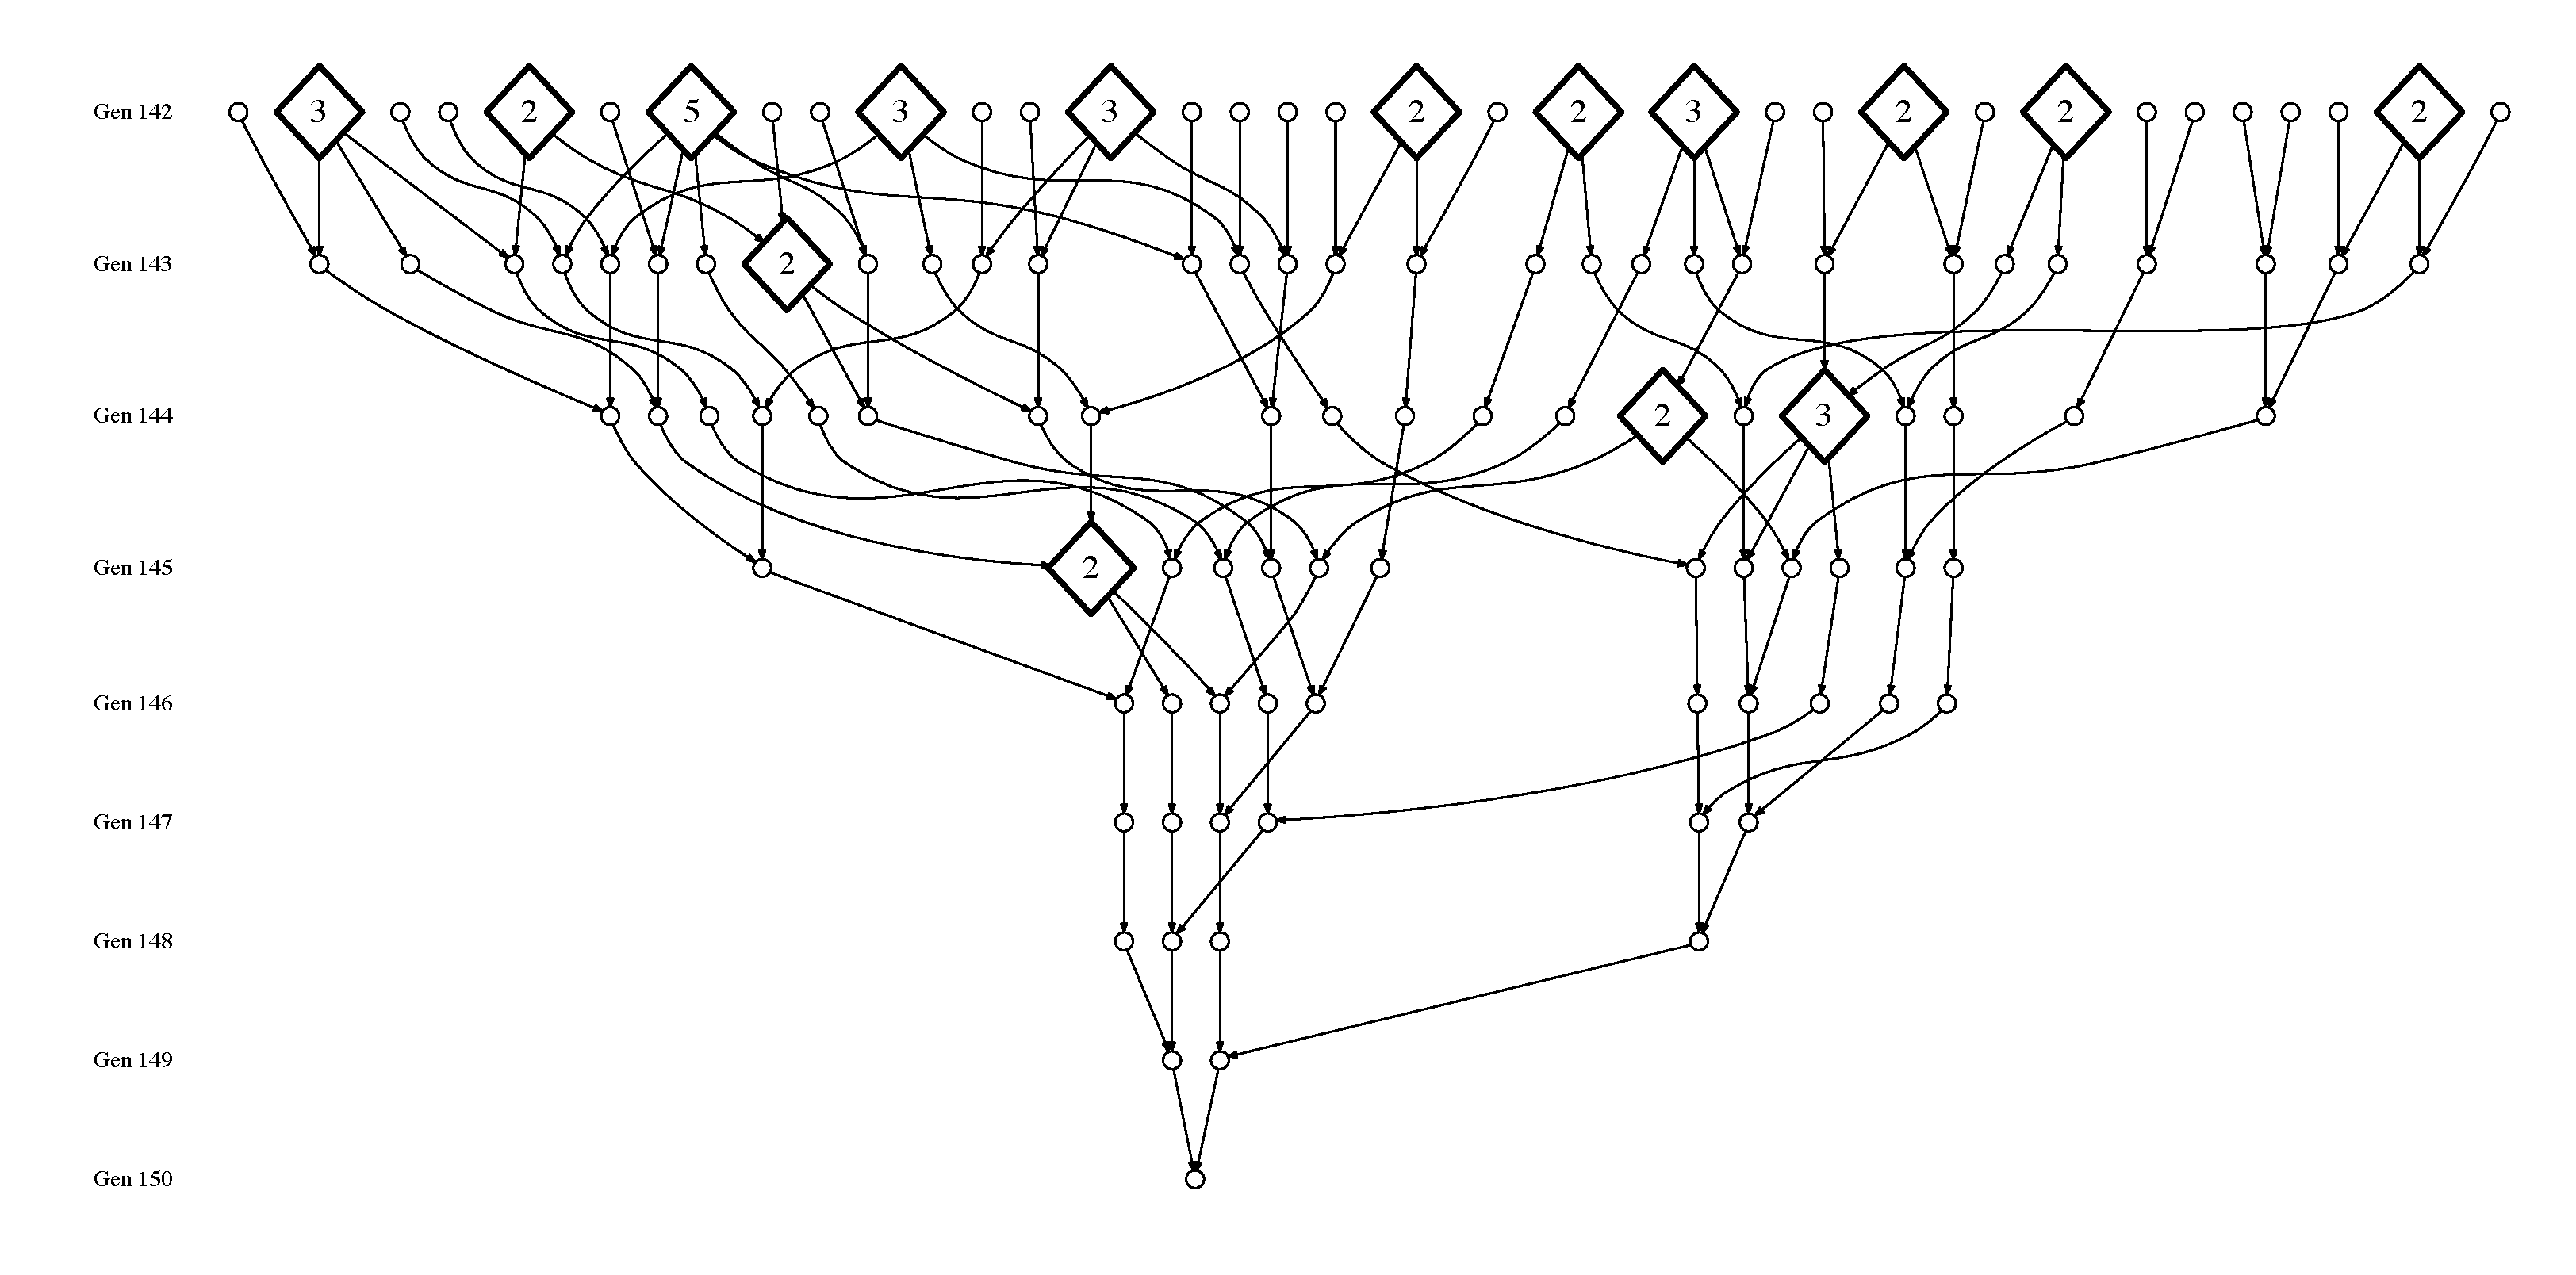
\includegraphics[width=\columnwidth]{figures/ancestors_of_winner_rswn_tourney_run74_9gens.pdf}
	\caption{Ancestry of the sole ``winners'' from run 74 of tournament selection, 
		replace-space-with-newline. The few nodes with more than one offspring that is an ancestor of the winner
		are marked with diamonds containing the number of children (in this graph) for that node. Most of those
		nodes had additional children, not pictured in the figure, that are not ancestors of the winning individual.)}
	\label{fig:winnerAncestorsTourneyRun74}
\end{sidewaysfigure}

In addition to studying lexicase selection, we wanted to collect data from replace-space-with-new-line 
with tournament selection in order to compare lexicase versus tournament. As previously noted in 
Section~\ref{sec:lexicaseRun}, lexicase  produced at least one individual with an error of zero in 
55 of 100 runs while tournament selection only produced 13 of 100 successful runs. Of these 13 
successful tournament runs, we selected one run to study.

An immediate difference that we notice between the lexicase and tournament runs was the number of 
individuals that solved the problem in the final generation. In lexicase, there were 45 different 
individuals that solved the problem while there was only a single individual in the tournament 
run that had an total error of zero across all the test cases.

Figure \ref{fig:winnerAncestorsTourneyRun74} shows the ancestry of the winning individual from 
generation 150 back to generation 145. It was not possible to show individuals farther back than 
generation 145 because of an interesting property of tournaments. Table~\ref{table:branching} shows 
the number of parents n generations away that contributed to the development of the winning individuals. 
The further away from the winning individual, the number of parents that contributed to the winner 
in tournament selection increased rapidly. In contrast, lexicase grew much more slowly, presumably 
due in part to the fact that in lexicase some parents produced a surprisingly large number of children; 
at 10 generations back, there were approximately three times the number of contributing parents in 
tournament as lexicase. Another possible contribution to this asymmetry is a difference in the role of
mutations under lexicase; that question is beyond the scope of this chapter, however.

\begin{table}%
	\centering
	\caption{Two examples of the impact of selection on evolutionary dynamics in the two explored runs. Table~\subref{table:branching} lists the number of parents contributing to a winning individual $n$ generations away for both the 
		lexicase and tournament runs explored in this paper. The top row, for example, indicates that in the lexicase run
		there were 58 distinct ancestors of a winning individual 18 generations before the discovery of a winner, and in
		the tournament run there were 297 distinct ancestors 18 generations before the discovery of a winner. 
		Table~\subref{table:numChildren} lists the 18 most fecund individuals across the entirity of each of the lexicase and tournament selection runs.}
	\label{tab:big}
	\subtable[]{
		\label{table:branching}%
		\begin{tabular}{rrr}
			& \multicolumn{2}{c}{Number of ancestors} \\
			$n$ & $\quad$ Lexicase & $\quad$ Tournament \\
			\hline\noalign{\smallskip}
			18 & 58 & 297 \\
			17 & 52 & 236 \\
			16 & 46 & 180 \\
			15 & 49 & 152 \\
			14 & 45 & 209 \\
			13 & 46 & 212 \\
			12 & 41 & 146 \\
			11 & 29 & 97 \\
			10 & 22 & 63 \\
			9 & 14 & 42 \\
			8 & 14 & 33 \\
			7 & 10 & 30 \\
			6 & 9 & 20 \\
			5 & 7 & 13 \\
			4 & 6 & 10 \\
			3 & 7 & 6 \\
			2 & 6 & 4 \\
			1 & 4 & 2 \\
		\end{tabular}		
		}
		\qquad
	\subtable[]{
		\label{table:numChildren}
		\begin{tabular}{rrr}
			& \multicolumn{2}{c}{Number of children} \\
			Rank in run & $\quad$ Lexicase & $\quad$ Tournament \\
			\hline\noalign{\smallskip}
			1 & 934 & 24 \\
			2 & 657 & 23 \\
			3 & 594 & 23 \\
			4 & 590 & 21 \\
			5 & 433 & 20 \\
			6 & 326 & 20 \\
			7 & 297 & 19 \\
			8 & 294 & 19 \\
			9 & 285 & 19 \\
			10 & 283 & 18 \\
			11 & 279 & 18 \\
			12 & 271 & 18 \\
			13 & 234 & 18 \\
			14 & 220 & 18 \\
			15 & 212 & 18 \\
			16 & 205 & 18 \\
			17 & 203 & 18 \\
			18 & 202 & 17 \\
%			19 & 200 & 17 \\
%			20 & 189 & 17 \\
		\end{tabular}
		}%
\end{table}

Another major difference was the selection pressure of the two selection mechanisms. In lexicase 
selection, one parent can dominate the selection if it performs well for a majority of the test 
cases as we saw in section~\ref{sec:surprisingFecundity} where individual 86:261 was a parent for 
all but 76 individuals in the final generation. However, tournament selection can never 
impose such a strong selection pressure. Throughout the entire run,
the most a single parent in the tournament selection run ever produced was 24 children 
(see Table~\ref{table:numChildren}), and all of the 18 most prolific parents produced between 17
and 24 offspring. Compare this to lexicase selection, where all of the 18 top parents produced over 
200. This extreme difference in selection pressure may also help explain the observation that the 
differences in the branching factor of the two ancestry trees.

Beside selection pressure, we noticed another crucial difference between the types of individuals 
selected for reproduction. With tournament selection, the primary bias is towards individuals that 
have the lowest total error. However, this is not the case in lexicase.  As long as an individual 
performs extremely well for some cases (but not necessarily all), it is still possible to be selected for 
reproduction. In Table~\ref{table:winnerFitnesses}, individual 85:086 has an error of 100,000. 
This late into the run, it would be very unlikely that tournament would select this individual to 
reproduce. In fact, we see this in the tournament run, where every ancestor of the winner in the
last six generations of the
has a total error of either 83 or 132. Additionally, across all individuals chosen
as parents in the last 20 generations (regardless of whether they were an ancestor of the winner), 
there were as few as one and at most five distinct total errors within each generation. 
This suggests that tournament selection keeps
mutating and recombining the best individuals together until it manages, essentially by accident, to produce an improved 
child. Lexicase, on the other hand, maintains a much more diverse population and appears to somehow leverage that
diversity to continue to discover improvements. One possibility (which needs additional exploration) is that under lexicase 
the system is able to combine components of programs that solve different test cases in a way that allows it
to construct improved offspring.

\marginpar{Deal with these bullets.}
\begin{itemize}
	\item Tournament winner was produced with alternation and uniform-mutation (mutation could have possibly caused the problem to be solved)
	\item Many alternations and mutations in the last generations along the winning ancestry produced children that had 0 error difference from the better parent. 
\end{itemize}


%Crossover mutation events get us to end?

%Branching

%Table of 20 with most offspring for both 
%more various numbers in table

\section{A few cumulative results}
\label{sec:cumulativeResults}

The bulk of this chapter has focused on exploring two specific successful runs on the replace-space-with-newline problem,
one using lexicase selection, and one using tournament selection. To better understand how well this application of graph
databases scales, we also created two larger cumulative databases, each containing the complete genealogical record for all 
100 runs on replace-space-with-newline using, respectively, lexicase and tournament selection. Given these cumulative 
databases, we were then able to do broad queries against those collections of runs. These were typically inspired by 
observations from the explorations of individual runs, with the broader queries helping us understand to what degree an 
observation in an individual run was representative of behavior in other runs.

An obvious question, for example, is how unusual is the individual we discovered in Section~\ref{sec:surprisingFecundity} 
that had 934 offspring? Was that an aberration, or are these kinds of hyper-selected and hyper-fecund individuals a
regular occurrence when using lexicase selection? Querying the combined database revealed that there were 71 individuals
in the 100 lexicase runs that were selected more than 900 times, where the average number of selections in a given 
generation was 1,700. So each of these 71 individuals received over half the total selections in its generation, and 
consequently had numerous offspring; all had over 700 offspring out of the 1,000 created for the next generation. 22 of
those 71 individuals had over 900 offspring, with the biggest winners being two individuals that had 990 and 991 
offspring, respectively, after being selected over 1,600 times each. 

These 71 individuals clearly represent a very small fraction of the over 18 million nodes encapsulated in our 100 lexicase
runs. 50 of
the 100 runs, however, had at least one of these hyper-selected individuals with over 900 selections, so this kind of 
hyper-selection is clearly a common component of the dynamics of these lexicase runs. This sort of hyper-selection 
has a profound impact on the dynamics of a run, as almost every individual in the subsequent generation is a child of
the hyper-selected individual, and due to self-crosses that individual is often the \emph{only} parent of those children. Thus
the genetics of that individual are likely to have an enormous influence on the make-up of the next generation, creating
what is in effect a substantial population bottleneck. So while those 71 individuals only represent a tiny proportion of
the cumulative population, they're likely to have a tremendous impact on the run dynamics, so the ability to indentify and
examine these individuals is potentially very informative.

One of the other surprises from our earlier exploration is how ``unfit'' some of those highly selected individuals were when
viewed through the lens of total error. Turning now to these cumulative results, we find that 15 of these 71 hyper-selected
individuals had total error at or below 10, and so would likely be selected by tournament selection (although never more 
than a few dozen times). On the other end of the spectrum, however, 7 of these 71 hyper-selected individuals had total 
error over 3,000 and would have been \emph{extremely} unlikely to ever be chosen using tournament selection. So here
again we see a substantial difference between the dynamics of lexicase and tournament selection, especially given the
impact these hyper-selected individuals have on their runs.

\section{So what did we learn in all this?}
\label{sec:whatDidWeLearn}

In this chapter we've illustrated the potential of graph databases such as Neo4j as tools for exploring 
and analyzing some of the rich matrix of low-level events that ultimately make up any evolutionary
computation run. Here we've used graph databases as a new kind of ``lab bench'' instrument, allowing us to
zoom in and capture the details of potentially crucial moments in our GP runs.

This has exposed surprising and potentially important properties of lexicase selection. These properties will 
hopefully help us better understand dynamics of runs using lexicase, and why those runs are frequently more 
successful than runs using tournament selection. A key goal in the original design of lexicase selection 
\citep{Helmuth:2015:ieeeTEC} was to increase and maintain diversity in GP runs which, as \citep{Helmuth:2015:GPTP}
shows, does appear to be the case, with lexicase generally leading to more diversity
than either tournament selection or implicit fitness sharing. One would, however, typically consider hyper-selection
and the consequent population bottlenecks to be the enemy of diversity, so our discovery of a pattern of
individuals being selected hundreds, and sometimes even \emph{thousands}, of times was at the very least noteworthy
and worthy of further study.

A key risk in this sort of narrow examination of the details of runs is that one might mistake a single or small
number of observations for a pattern. Thus there will always be a need for the summary results provided by tables, 
plots, and other statistical tools. The kind of exploration we've demonstrated here will ultimately have
to be used in conjunction with those statistical tools; discoveries in ``digs'' such as these can raise questions 
and suggest hypotheses that can then be supported or refuted through the use of more ``traditional'' studies.

One other concern is how well our use of graph databases can scale. Databases for individual runs are quite tractable,
and can be populated and explored using basic off-the-shelf computers. Combing multiple runs, however, presents a
number of challenges. The database containing the 100 lexicase runs, for example, contained over 18 million nodes 
and over 25 million edges, with the full Neo4j database weighing in at 18GB. The database combining the 100 tournament
runs was even larger because most of the runs went the full 300 generations: over 28 million nodes, over 48 million edges,
and a database of over 31GB. That said, these databases runs reasonably on stock desktop 
hardware, which is how all the results presented here were generated. We'd quickly start to need more specialized
infrastructure to scale up further if, for example, we wanted to combine the 
lexicase and tournament selection runs into a single database containing the history of those 200 runs, or combining
the results of runs on multiple problems. We have data from thousands of runs \citep{Helmuth:2015:GPTP}, but bringing
that together in a single database is clearly infeasible using these tools. An alternative to this approach would be
to have a host of database engines on a cluster, each serving a subset of related data, and then providing tools
that would allow queries to be run across all these endpoints, aggregating those results into a single response. Version
1.1 of the SPARQL query language \citep{wiki:SPARQL}, for example, includes support for queries across multiple endpoints
and could potentially be used to run queries across large distributed datasets.

\begin{acknowledgement}
	Thanks to the members of the Hampshire College Computational Intelligence Lab and M. Kirbie Dramdahl
	at the University of Minnesota, Morris, for discussions that 
	helped to improve the work described in this paper. Thanks also to Josiah Erikson for systems support, and to 
	Hampshire College for support for the Hampshire College Institute for Computational Intelligence. 
	This material is based upon work supported by the National Science Foundation under Grants No. 1017817, 
	1129139, and 1331283. Any opinions, findings, and conclusions or recommendations expressed in this 
	publication are those of the authors and do not necessarily reflect the views of the National 
	Science Foundation.	
	
	We are very grateful to all the participants in the 2015 Genetic Programming Theory and Practice (GPTP)
	workshop for their enthusiasm, ideas, and support. In particular we'd like to thank William Tozier 
	for all manner of suggestions and feedback, and in particular for helping us understand
	the connection between our work and the Pickering's idea of the ``mangle of practice''. Krzysztof Krawiec
	provided a number of valuable suggestions based on an early draft. Steven Gustafson suggested that we
	look into SPARQL and triplestore databases as an alternative to Neo4j, an interesting idea we haven't had time to
	explore fully. Finally, thanks to the GPTP organizers; without their hard work none of those other valuable
	conversations would have occurred.
\end{acknowledgement}

\bibliographystyle{spbasic}
\bibliography{gp-bibliography,chapter}
